\chapter{$n\equiv 0,1\pmod{14}$}
\label{intro_chapter}

In this section, we use established graph labeling techniques to construct the $G$-decompositions of $K_n$ when $n \equiv 0 \textrm{ or } 1 \pmod{14}$. 



\begin{definition}[(Rosa \cite{bib:rosa})] \label{def:rho} 
 Let $G$ be a graph with $m$ edges.  A \textit{$\rho$-labeling} of $G$ is an injection $f: V(G) \rightarrow \{0,1,2, \dots, 2m\}$ that induces a bijective \textit{length function $\ell: E(G) \rightarrow \{1,2, \dots, m\}$} where 
    $$
    \ell(uv) = \text{min}\{|f(u)-f(v)|,2m+1-|f(u)-f(v)|\},
    $$
for all  $uv \in E(G)$.
\end{definition}

Rosa showed that a $\rho$-labeling of a graph $G$ with $m$ edges and a cyclic $G$-decomposition of $K_{2m+1}$ are equivalent, which the next thm shows. Later, Rosa, his students, and colleagues began considering more restrictive types of $\rho$-labeling to address decomposing complete graphs of more orders. Definitions of these labelings and related results follow.

\begin{thm}[(Rosa \cite{bib:rosa})]\label{thm:Rhosa}  
Let $G$ be a graph with $m$ edges.  There exists a cyclic $G$-decomposition of $K_{2m+1}$ if and only if $G$ admits a $\rho$-labeling.
\end{thm}

\begin{definition}[(Rosa \cite{bib:rosa})] \label{def:sigma} 
A $\sigma$-labeling of a graph $G$ is a $\rho$-labeling such that $\ell(uv) = |f(u) - f(v)|$ for all $uv \in E(G).$
\end{definition}

\begin{definition}[(El-Zanati, Vanden Eynden \cite{cyclicbipart})] \label{def:rho and sigma ordered def} 
A $\rho$- or $\sigma$-labeling of a bipartite graph $G$ with bipartition $(A,B)$ is called an \emph{ordered} $\rho$- or $\sigma$-labeling and denoted $\rho^+,\sigma^+$, respectively, if $f(a) < f(b)$ for each edge $ab$ with $a \in A$ and $b \in B$.
\end{definition}

\begin{thm}[(El-Zanati, Vanden Eynden \cite{cyclicbipart})] \label{thm:rho plus}
Let $G$ be a graph with $m$ edges which has a $\rho^+$-labeling.  Then $G$ decomposes $K_{2mk+1}$ for all positive integers $k$.
\end{thm}

\begin{definition}[(Freyberg, Tran \cite{tran})] \label{def:sigma plus minus} 
A $\sigma^{+-}$-\emph{labeling} of a bipartite graph $G$ with $m$ edges and bipartition $(A,B)$ is a $\sigma^+$-labeling with the property that $f(a) - f(b) \neq m$ for all $a \in A$ and $b \in B$, and $f(v) \not\in \{2m,2m-1\}$ for any $v\in V(G)$.
\end{definition}

\begin{thm}[(Freyberg, Tran \cite{tran})] \label{thm:sigma plus minus}
Let $G$ be a graph with $m$ edges and a $\sigma^{+-}$-labeling such that the edge of length $m$ is a pendant. Then there exists a $G$-decomposition of both $K_{2mk}$ and $K_{2mk+1}$ for every positive integer $k$.
\end{thm}

Figure \ref{fig:sigma plus minus} gives a $\sigma^{+-}$-labeling of every forest with 7 edges. The vertex labels of each connected component with $k$ vertices are given as a $k$-tuple, $(v_1,\dots ,v_k)$ corresponding to the vertices $v_1, \dots, v_k$ given in Figure \ref{fig:catalog}. We leave it to the reader to infer the bipartition $(A,B)$. 
\begin{example}
    A $\sigma^{+-}$-labeling of $\mathbf{T_{6}^{6}}\sqcup 2\mathbf{T_{2}^{1}}$ is shown in Figure \ref{fig:sigma label ex}. The vertices labeled $1,2$ and $9$ belong to $A$, and the others belong to $B$. The lengths of each edge are indicated on the edge.
    \begin{figure}[H]
        \centering
        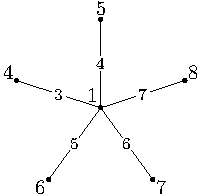
\includegraphics[scale=1.0]{standalone/sigma label ex1.pdf}
         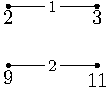
\includegraphics[scale=1.0]{standalone/sigma label ex2.pdf}
        \caption{$\sigma^{+-}$-labeling of $\mathbf{T_{6}^{6}}\sqcup 2\mathbf{T_{2}^{1}}$}
        \label{fig:sigma label ex}
    \end{figure}
\end{example}
 The labelings given in Figure \ref{fig:sigma plus minus} along with thm \ref{thm:sigma plus minus} are enough to prove the following thm. \newpage 

 %\begin{figure}[H]
 %   \centering
 %   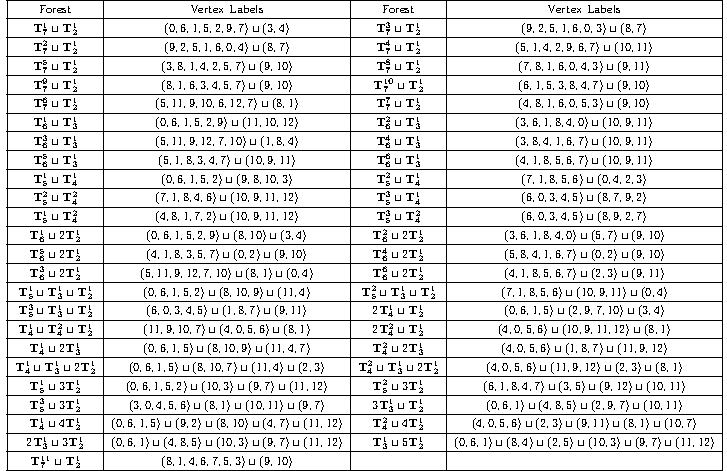
\includegraphics[scale=1.1]{0,1(mod 14).pdf}
 %   \caption{$\sigma^{+-}$-labelings for forests with 7 edges}
 %  \label{fig:sigma plus minus}
%\end{figure}
% or

\resize{\documentclass{article}

\usepackage{graphicx}
\usepackage{array}
\usepackage{standalone}
\usepackage{amsmath}
\usepackage{longtable} % Ensures column widths persist after page breaks
\usepackage{caption} % Allows captioning outside figures

\begin{document}
\renewcommand{\arraystretch}{1.2} % Keep row spacing consistent
\setlength{\tabcolsep}{8pt} % Keep column spacing consistent
{\def\arraystretch{1}%
    \begin{longtable}{|c|c|} % Forces same width after first page
        \hline
        Forest & Vertex Labels \\
        \hline
            $\mathbf{T_{7}^{1}} \sqcup \mathbf{T_{2}^{1}}$ & \begin{tabular}{@{}l@{}} $(0,6,1,5,2,9,7)\sqcup(3,4)$ \end{tabular} \\ \hline
    $\mathbf{T_{7}^{3}} \sqcup \mathbf{T_{2}^{1}}$ & \begin{tabular}{@{}l@{}} $(9,2,5,1,6,0,3)\sqcup(8,7)$ \end{tabular} \\ \hline
    $\mathbf{T_{7}^{2}} \sqcup \mathbf{T_{2}^{1}}$ & \begin{tabular}{@{}l@{}} $(9,2,5,1,6,0,4)\sqcup(8,7)$ \end{tabular} \\ \hline
    $\mathbf{T_{7}^{4}} \sqcup \mathbf{T_{2}^{1}}$ & \begin{tabular}{@{}l@{}} $(5,1,4,2,9,6,7)\sqcup(10,11)$ \end{tabular} \\ \hline
    $\mathbf{T_{7}^{5}} \sqcup \mathbf{T_{2}^{1}}$ & \begin{tabular}{@{}l@{}} $(3,8,1,4,2,5,7)\sqcup(9,10)$ \end{tabular} \\ \hline
    $\mathbf{T_{7}^{8}} \sqcup \mathbf{T_{2}^{1}}$ & \begin{tabular}{@{}l@{}} $(7,8,1,6,0,4,3)\sqcup(9,11)$ \end{tabular} \\ \hline
    $\mathbf{T_{7}^{9}} \sqcup \mathbf{T_{2}^{1}}$ & \begin{tabular}{@{}l@{}} $(8,1,6,3,4,5,7)\sqcup(9,10)$ \end{tabular} \\ \hline
    $\mathbf{T_{7}^{10}} \sqcup \mathbf{T_{2}^{1}}$ & \begin{tabular}{@{}l@{}} $(6,1,5,3,8,4,7)\sqcup(9,10)$ \end{tabular} \\ \hline
    $\mathbf{T_{7}^{6}} \sqcup \mathbf{T_{2}^{1}}$ & \begin{tabular}{@{}l@{}} $(5,11,9,10,6,12,7)\sqcup(8,1)$ \end{tabular} \\ \hline
    $\mathbf{T_{7}^{7}} \sqcup \mathbf{T_{2}^{1}}$ & \begin{tabular}{@{}l@{}} $(4,8,1,6,0,5,3)\sqcup(9,10)$ \end{tabular} \\ \hline
    $\mathbf{T_{6}^{1}} \sqcup \mathbf{T_{3}^{1}}$ & \begin{tabular}{@{}l@{}} $(0,6,1,5,2,9)\sqcup(11,10,12)$ \end{tabular} \\ \hline
    $\mathbf{T_{6}^{2}} \sqcup \mathbf{T_{3}^{1}}$ & \begin{tabular}{@{}l@{}} $(3,6,1,8,4,0)\sqcup(10,9,11)$ \end{tabular} \\ \hline
    $\mathbf{T_{6}^{3}} \sqcup \mathbf{T_{3}^{1}}$ & \begin{tabular}{@{}l@{}} $(5,11,9,12,7,10)\sqcup(1,8,4)$ \end{tabular} \\ \hline
    $\mathbf{T_{6}^{4}} \sqcup \mathbf{T_{3}^{1}}$ & \begin{tabular}{@{}l@{}} $(3,8,4,1,6,7)\sqcup(10,9,11)$ \end{tabular} \\ \hline
    $\mathbf{T_{6}^{5}} \sqcup \mathbf{T_{3}^{1}}$ & \begin{tabular}{@{}l@{}} $(5,1,8,3,4,7)\sqcup(10,9,11)$ \end{tabular} \\ \hline
    $\mathbf{T_{6}^{6}} \sqcup \mathbf{T_{3}^{1}}$ & \begin{tabular}{@{}l@{}} $(4,1,8,5,6,7)\sqcup(10,9,11)$ \end{tabular} \\ \hline
    $\mathbf{T_{5}^{1}} \sqcup \mathbf{T_{4}^{1}}$ & \begin{tabular}{@{}l@{}} $(0,6,1,5,2)\sqcup(9,8,10,3)$ \end{tabular} \\ \hline
    $\mathbf{T_{5}^{2}} \sqcup \mathbf{T_{4}^{1}}$ & \begin{tabular}{@{}l@{}} $(7,1,8,5,6)\sqcup(0,4,2,3)$ \end{tabular} \\ \hline
    $\mathbf{T_{5}^{2}} \sqcup \mathbf{T_{4}^{2}}$ & \begin{tabular}{@{}l@{}} $(7,1,8,4,6)\sqcup(10,9,11,12)$ \end{tabular} \\ \hline
    $\mathbf{T_{5}^{3}} \sqcup \mathbf{T_{4}^{1}}$ & \begin{tabular}{@{}l@{}} $(6,0,3,4,5)\sqcup(8,7,9,2)$ \end{tabular} \\ \hline
    $\mathbf{T_{5}^{1}} \sqcup \mathbf{T_{4}^{2}}$ & \begin{tabular}{@{}l@{}} $(4,8,1,7,2)\sqcup(10,9,11,12)$ \end{tabular} \\ \hline
    $\mathbf{T_{5}^{3}} \sqcup \mathbf{T_{4}^{2}}$ & \begin{tabular}{@{}l@{}} $(6,0,3,4,5)\sqcup(8,9,2,7)$ \end{tabular} \\ \hline
    $\mathbf{T_{6}^{1}} \sqcup 2\mathbf{T_{2}^{1}}$ & \begin{tabular}{@{}l@{}} $(0,6,1,5,2,9)\sqcup(8,10)\sqcup(3,4)$ \end{tabular} \\ \hline
    $\mathbf{T_{6}^{2}} \sqcup 2\mathbf{T_{2}^{1}}$ & \begin{tabular}{@{}l@{}} $(3,6,1,8,4,0)\sqcup(5,7)\sqcup(9,10)$ \end{tabular} \\ \hline
    $\mathbf{T_{6}^{5}} \sqcup 2\mathbf{T_{2}^{1}}$ & \begin{tabular}{@{}l@{}} $(4,1,8,3,5,7)\sqcup(0,2)\sqcup(9,10)$ \end{tabular} \\ \hline
    $\mathbf{T_{6}^{4}} \sqcup 2\mathbf{T_{2}^{1}}$ & \begin{tabular}{@{}l@{}} $(5,8,4,1,6,7)\sqcup(0,2)\sqcup(9,10)$ \end{tabular} \\ \hline
    $\mathbf{T_{6}^{3}} \sqcup 2\mathbf{T_{2}^{1}}$ & \begin{tabular}{@{}l@{}} $(5,11,9,12,7,10)\sqcup(8,1)\sqcup(0,4)$ \end{tabular} \\ \hline
    $\mathbf{T_{6}^{6}} \sqcup 2\mathbf{T_{2}^{1}}$ & \begin{tabular}{@{}l@{}} $(4,1,8,5,6,7)\sqcup(2,3)\sqcup(9,11)$ \end{tabular} \\ \hline
    $\mathbf{T_{5}^{1}} \sqcup \mathbf{T_{3}^{1}} \sqcup \mathbf{T_{2}^{1}}$ & \begin{tabular}{@{}l@{}} $(0,6,1,5,2)\sqcup(8,10,9)\sqcup(11,4)$ \end{tabular} \\ \hline
    $\mathbf{T_{5}^{2}} \sqcup \mathbf{T_{3}^{1}} \sqcup \mathbf{T_{2}^{1}}$ & \begin{tabular}{@{}l@{}} $(7,1,8,5,6)\sqcup(10,9,11)\sqcup(0,4)$ \end{tabular} \\ \hline
    $\mathbf{T_{5}^{3}} \sqcup \mathbf{T_{3}^{1}} \sqcup \mathbf{T_{2}^{1}}$ & \begin{tabular}{@{}l@{}} $(6,0,3,4,5)\sqcup(1,8,7)\sqcup(9,11)$ \end{tabular} \\ \hline
    $2\mathbf{T_{4}^{1}} \sqcup \mathbf{T_{2}^{1}}$ & \begin{tabular}{@{}l@{}} $(0,6,1,5)\sqcup(2,9,7,10)\sqcup(3,4)$ \end{tabular} \\ \hline
    $\mathbf{T_{4}^{1}} \sqcup \mathbf{T_{4}^{2}} \sqcup \mathbf{T_{2}^{1}}$ & \begin{tabular}{@{}l@{}} $(11,9,10,7)\sqcup(4,0,5,6)\sqcup(8,1)$ \end{tabular} \\ \hline
    $2\mathbf{T_{4}^{2}} \sqcup \mathbf{T_{2}^{1}}$ & \begin{tabular}{@{}l@{}} $(4,0,5,6)\sqcup(10,9,11,12)\sqcup(8,1)$ \end{tabular} \\ \hline
    $\mathbf{T_{4}^{1}} \sqcup 2\mathbf{T_{3}^{1}}$ & \begin{tabular}{@{}l@{}} $(0,6,1,5)\sqcup(8,10,9)\sqcup(11,4,7)$ \end{tabular} \\ \hline
    $\mathbf{T_{4}^{2}} \sqcup 2\mathbf{T_{3}^{1}}$ & \begin{tabular}{@{}l@{}} $(4,0,5,6)\sqcup(1,8,7)\sqcup(11,9,12)$ \end{tabular} \\ \hline
    $\mathbf{T_{4}^{1}} \sqcup \mathbf{T_{3}^{1}} \sqcup 2\mathbf{T_{2}^{1}}$ & \begin{tabular}{@{}l@{}} $(0,6,1,5)\sqcup(8,10,7)\sqcup(11,4)\sqcup(2,3)$ \end{tabular} \\ \hline
    $\mathbf{T_{4}^{2}} \sqcup \mathbf{T_{3}^{1}} \sqcup 2\mathbf{T_{2}^{1}}$ & \begin{tabular}{@{}l@{}} $(4,0,5,6)\sqcup(11,9,12)\sqcup(2,3)\sqcup(8,1)$ \end{tabular} \\ \hline
    $\mathbf{T_{5}^{1}} \sqcup 3\mathbf{T_{2}^{1}}$ & \begin{tabular}{@{}l@{}} $(0,6,1,5,2)\sqcup(10,3)\sqcup(9,7)\sqcup(11,12)$ \end{tabular} \\ \hline
    $\mathbf{T_{5}^{2}} \sqcup 3\mathbf{T_{2}^{1}}$ & \begin{tabular}{@{}l@{}} $(6,1,8,4,7)\sqcup(3,5)\sqcup(9,12)\sqcup(10,11)$ \end{tabular} \\ \hline
    $\mathbf{T_{5}^{3}} \sqcup 3\mathbf{T_{2}^{1}}$ & \begin{tabular}{@{}l@{}} $(3,0,4,5,6)\sqcup(8,1)\sqcup(10,11)\sqcup(9,7)$ \end{tabular} \\ \hline
    $3\mathbf{T_{3}^{1}} \sqcup \mathbf{T_{2}^{1}}$ & \begin{tabular}{@{}l@{}} $(0,6,1)\sqcup(4,8,5)\sqcup(2,9,7)\sqcup(10,11)$ \end{tabular} \\ \hline
    $\mathbf{T_{4}^{1}} \sqcup 4\mathbf{T_{2}^{1}}$ & \begin{tabular}{@{}l@{}} $(0,6,1,5)\sqcup(9,2)\sqcup(8,10)\sqcup(4,7)\sqcup(11,12)$ \end{tabular} \\ \hline
    $\mathbf{T_{4}^{2}} \sqcup 4\mathbf{T_{2}^{1}}$ & \begin{tabular}{@{}l@{}} $(4,0,5,6)\sqcup(2,3)\sqcup(9,11)\sqcup(8,1)\sqcup(10,7)$ \end{tabular} \\ \hline
    $2\mathbf{T_{3}^{1}} \sqcup 3\mathbf{T_{2}^{1}}$ & \begin{tabular}{@{}l@{}} $(0,6,1)\sqcup(4,8,5)\sqcup(10,3)\sqcup(9,7)\sqcup(11,12)$ \end{tabular} \\ \hline
    $\mathbf{T_{3}^{1}} \sqcup 5\mathbf{T_{2}^{1}}$ & \begin{tabular}{@{}l@{}} $(0,6,1)\sqcup(8,4)\sqcup(2,5)\sqcup(10,3)\sqcup(9,7)\sqcup(11,12)$ \end{tabular} \\ \hline
    \end{longtable}%
}
\label{fig:sigma plus minus}
\vspace{-4mm}
\begin{center}
    \captionof{figure}{$\sigma^{+-}$-labelings for forests with 7 edges}
\end{center}

\end{document}}{}

\begin{thm}\label{thm:0 or 1 mod 14}
    Let $F$ be a forest with $7$ edges. There exists an $F$-decomposition of $K_n$ whenever $n \equiv 0 \; \textrm{or} \; 1 \pmod{14}.$
\end{thm}
\begin{proof}
    The proof follows from thm \ref{thm:sigma plus minus} and the labelings given in Figure \ref{fig:sigma plus minus}.
\end{proof}